\section{Warum p2p?}
    Das vorausgegangen Projekt einer Verbindungskonfiguration von IoT-Geräten \linebreak \cite{aiProject} hat gezeigt, dass eine initiale p2p Verbindung aufgebaut werden muss, um eine Wi-Fi Verbindung konfigurieren zu können. Eine direkte Verbindung zwischen zwei Endgeräten ist nötig, wenn Daten zwischen Diesen ausgetauscht werden sollen und keine Verbindung über ein gemeinsames Netzwerk oder einen Server stattfinden kann oder soll. 
    
    - Warum p2p

    - Präzisierung IoT - Internet of Things
    
Das Zustandsmodell \reffig{p2p:state} eines p2p Verbindungsaufbaus lässt sich aus Sicht der beteiligten Geräte soweit vereinfachen, dass lediglich fünf von außen beobachtbare Zustände für eine erfolgreiche Nutzung einer p2p Verbindung relevant sind.
    
	\begin{figure}[ht]
         \centering
	      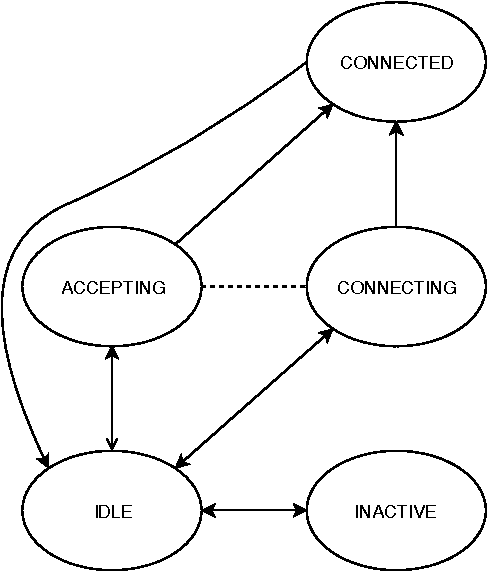
\includegraphics[width=0.5\textwidth]{p2p-State.pdf}
    	   \caption[Zustandsmodell eines p2p Verbindungsaufbaus]{Das Zustandsmodell eines p2p Verbindungsaufbaus zeigt die von außen beobachtbaren Zustände für eine erfolgreiche Nutzung einer p2p Verbindung. } \label{p2p:state}
	\end{figure}       
    
    \subsection{Services}
    - Definition eines Services
    
    - Anbieten eines Services als Client/Server-Modell
    
    \subsection{Servicestabilität (Todo: entfällt eventuell)}
    - API Versionierung
    
    - Absichern von Änderungen durch Contract-Driven-Development
    
    - Integrationstests
    \subsection{Netzwerktypen}
		- LAN, WAN, etc.
		
		- ad hoc, Stern-basiert, Bus-basiert
